\documentclass{article}
%\documentclass[a4paper,twoside]{article}
%\documentclass[a4paper]{article}
\usepackage{epsfig}
\usepackage{subfigure}
\usepackage{calc}
\usepackage{amssymb}
\usepackage{amstext}
\usepackage{amsmath}
\usepackage{amsthm}
\usepackage{multicol}
\usepackage{pslatex}
%\usepackage{apalike}
\usepackage{url}
\usepackage{hyperref}
\usepackage{placeins}


\usepackage{graphicx}
\usepackage{makeidx}  % allows for indexgeneration
\usepackage{epsfig}
\usepackage{subfigure}
\usepackage{calc}
\usepackage{amssymb}
\usepackage{multicol}
%\usepackage{apalike}
\usepackage{graphicx}
\usepackage{listings}
\usepackage{url}
\newtheorem{observation}{Observation}
\usepackage{zed}
\usepackage{algpseudocode}

% and for multiplicity 

\def\optional{0{\upto}1}
\def\mandatory{1{\upto} 1}
\def\many{0{\upto}*}

% partial ordering on constraints

\def\Cimplies{\mathrel{\implies_c}}
\def\Ciff{\mathrel{\iff_c}}

%  partial ordering on text

\def\Timplies{\mathrel{\implies_t}}
\def\Tiff{\mathrel{\iff_t}}

% and conjunction 
\def\Tand{\mathrel{\land_t}}
\def\TAnd{\mathop{\land_t}}
% our globalised version of the defining relations
\def\refines{\mathrel{refines}}
\def\newVersionOf{\mathrel{newVersionOf}}
\def\extends{\mathrel{extends}}
\def\contains{\mathrel{contains}}
% we may have \sqsubseteq and \gg when it comes to analysis 
% our two status values 
\def\draft{\mathsf{draft}}
\def\final{\mathsf{final}}
%load any additional packages

\newcommand\Algphase[1]{%
	\vspace*{-.7\baselineskip}\Statex\hspace*{\dimexpr-\algorithmicindent-2pt\relax}\rule{\textwidth}{0.4pt}%
	\Statex\hspace*{-\algorithmicindent}\textbf{#1}%
	\vspace*{-.7\baselineskip}\Statex\hspace*{\dimexpr-\algorithmicindent-2pt\relax}\rule{\textwidth}{0.4pt}%
}


%\usepackage{SCITEPRESS}  % Please add other packages that you may need BEFORE the SCITEPRESS.sty package.

\begin{document}
	%
%	\frontmatter          % for the preliminaries
	%
	\pagestyle{headings}  % switches on printing of running heads
	\title{Healthcare Data Research - Metadata Federation}
	
	\author{Jim Davies, Gerry Reilly,  David Milward, \\ Adam Milward, Ashutosh Tripathi, James Welch}
	
	
	\maketitle
	
	\begin{abstract}
	This document outlines the way in which health data can be registered, identified and classified by its metadata, and how the metadata can be stored in registries which can be federated to help researchers find relevant data quickly and efficiently. These guidelines are based on existing standards such as ISO11179, DCAT and XMPP as well as a number of other tried and tested internet engineering standards and practises.	\end{abstract}
	%
	
	%
	\section{Scope}
	This Technical Report describes the proposed metadata standard for registration and federation of UK healthcare research datasets. Some aspects have been based on or derived from existing standards such as DCAT (\url{https://www.w3.org/TR/vocab-dcat-2/#bib-vocab-dcat-20140116}),DCAT2 (\url{https://www.w3.org/TR/vocab-dcat-2/#introduction}) and ISO11179 (see \url{http://metadata-standards.org/11179/}).
	
	The specification is split into 3 parts: a) the first part covers metadata required to manage data catalogues, and is descriptive in content, b) the second part covers technical metadata, and is based on a formal (or mathematical) metamodel of data, c) the third part covers the federation of healthcare metadata.
	
	
	
	\begin{enumerate}
		\item A need for a Data Dictionary that defines enterprise data (not “Standards”) in which a name,
definition, datatype and enumeration if present, need to be made available in machine readable
and human readable format for:
	\begin{enumerate}
		\item Data sharing
		\item Semi-automated customization of data collection tools
	\end{enumerate}
		\item A need for metadata specifications to be made available in machine readable format to support data mapping and transformation.
		\item A data catalogue that can be published and linked to specifications for its data elements	
	\end{enumerate}


	
\section{Normative References}

The following documents, in whole or in part, are normatively referenced in this document and are indispensable for its application. For dated references, only the edition cited applies. For undated references, the latest edition of the referenced document (including any amendments) applies.
[ISO/IEC 11179 – 1], Information technology — Metadata registries (MDR) — Part 1: Framework

[ISO/IEC 11179 – 3], Information technology — Metadata registries (MDR) — Part 3: Registry metamodel and basic attributes.

[BASE64],	Josefsson, S., “The Base16, Base32, and Base64 Data Encodings,” RFC 4648, October 2006 (TXT).

%[CHANNEL]	Williams, N., “On the Use of Channel Bindings to Secure Channels,” RFC 5056, November 2007 (TXT).
%
%[CHANNEL-TLS]	Altman, J., Williams, N., and L. Zhu, “Channel Bindings for TLS,” RFC 5929, July 2010 (TXT).
%
%[CHARSETS]	Alvestrand, H., “IETF Policy on Character Sets and Languages,” BCP 18, RFC 2277, January 1998 (TXT, HTML, XML).
%
%[DNS-CONCEPTS]	Mockapetris, P., “Domain names - concepts and facilities,” STD 13, RFC 1034, November 1987 (TXT).
%
%[DNS-SRV]	Gulbrandsen, A., Vixie, P., and L. Esibov, “A DNS RR for specifying the location of services (DNS SRV),” RFC 2782, February 2000 (TXT).
%
%[IPv6-ADDR]	Kawamura, S. and M. Kawashima, “A Recommendation for IPv6 Address Text Representation,” RFC 5952, August 2010 (TXT).
%
%[KEYWORDS]	Bradner, S., “Key words for use in RFCs to Indicate Requirement Levels,” BCP 14, RFC 2119, March 1997 (TXT, HTML, XML).
%
%[LANGMATCH]	Phillips, A. and M. Davis, “Matching of Language Tags,” BCP 47, RFC 4647, September 2006 (TXT).
%
%[LANGTAGS]	Phillips, A. and M. Davis, “Tags for Identifying Languages,” BCP 47, RFC 5646, September 2009 (TXT).
%
%[OCSP]	Myers, M., Ankney, R., Malpani, A., Galperin, S., and C. Adams, “X.509 Internet Public Key Infrastructure Online Certificate Status Protocol - OCSP,” RFC 2560, June 1999 (TXT).
%
%[PKIX]	Cooper, D., Santesson, S., Farrell, S., Boeyen, S., Housley, R., and W. Polk, “Internet X.509 Public Key Infrastructure Certificate and Certificate Revocation List (CRL) Profile,” RFC 5280, May 2008 (TXT).
%
%[PKIX-ALGO]	Jonsson, J. and B. Kaliski, “Public-Key Cryptography Standards (PKCS) \#1: RSA Cryptography Specifications Version 2.1,” RFC 3447, February 2003 (TXT).
%
%[PKIX-SRV]	Santesson, S., “Internet X.509 Public Key Infrastructure Subject Alternative Name for Expression of Service Name,” RFC 4985, August 2007 (TXT).
%
%[PLAIN]	Zeilenga, K., “The PLAIN Simple Authentication and Security Layer (SASL) Mechanism,” RFC 4616, August 2006 (TXT).
%
%[RANDOM]	Eastlake, D., Schiller, J., and S. Crocker, “Randomness Requirements for Security,” BCP 106, RFC 4086, June 2005 (TXT).
%
%[SASL]	Melnikov, A. and K. Zeilenga, “Simple Authentication and Security Layer (SASL),” RFC 4422, June 2006 (TXT).
%
%[SCRAM]	Newman, C., Menon-Sen, A., Melnikov, A., and N. Williams, “Salted Challenge Response Authentication Mechanism (SCRAM) SASL and GSS-API Mechanisms,” RFC 5802, July 2010 (TXT).
%
%[STRONGSEC]	Schiller, J., “Strong Security Requirements for Internet Engineering Task Force Standard Protocols,” BCP 61, RFC 3365, August 2002 (TXT).
%
%[TCP]	Postel, J., “Transmission Control Protocol,” STD 7, RFC 793, September 1981 (TXT).
%
%[TLS]	Dierks, T. and E. Rescorla, “The Transport Layer Security (TLS) Protocol Version 1.2,” RFC 5246, August 2008 (TXT).
%
%[TLS-CERTS]	Saint-Andre, P. and J. Hodges, “Representation and Verification of Domain-Based Application Service Identity within Internet Public Key Infrastructure Using X.509 (PKIX) Certificates in the Context of Transport Layer Security (TLS),” RFC 6125, March 2011.
%[TLS-NEG]	Rescorla, E., Ray, M., Dispensa, S., and N. Oskov, “Transport Layer Security (TLS) Renegotiation Indication Extension,” RFC 5746, February 2010 (TXT).
%
%[TLS-SSL2]	Turner, S. and T. Polk, “Prohibiting Secure Sockets Layer (SSL) Version 2.0,” RFC 6176, March 2011.
%[UNICODE]	The Unicode Consortium, “The Unicode Standard, Version 6.0,” 2010.
%
%[UTF-8]	Yergeau, F., “UTF-8, a transformation format of ISO 10646,” STD 63, RFC 3629, November 2003 (TXT).
%
%[URI]	Berners-Lee, T., Fielding, R., and L. Masinter, “Uniform Resource Identifier (URI): Generic Syntax,” STD 66, RFC 3986, January 2005 (TXT, HTML, XML).
%
%[X509]	International Telecommunications Union, “Information technology - Open Systems Interconnection - The Directory: Public-key and attribute certificate frameworks,” ITU-T Recommendation X.509, ISO Standard 9594-8, March 2000.
%[XML]	Maler, E., Yergeau, F., Sperberg-McQueen, C., Paoli, J., and T. Bray, “Extensible Markup Language (XML) 1.0 (Fifth Edition),” World Wide Web Consortium Recommendation REC-xml-20081126, November 2008 (HTML).
%
%[XML-GUIDE]	Hollenbeck, S., Rose, M., and L. Masinter, “Guidelines for the Use of Extensible Markup Language (XML) within IETF Protocols,” BCP 70, RFC 3470, January 2003 (TXT, HTML, XML).
%
%[XML-MEDIA]	Murata, M., St. Laurent, S., and D. Kohn, “XML Media Types,” RFC 3023, January 2001 (TXT).
%
%[XML-NAMES]	Thompson, H., Hollander, D., Layman, A., Bray, T., and R. Tobin, “Namespaces in XML 1.0 (Third Edition),” World Wide Web Consortium Recommendation REC-xml-names-20091208, December 2009 (HTML).
%
%[XMPP-ADDR]	Saint-Andre, P., “Extensible Messaging and Presence Protocol (XMPP): Address Format,” RFC 6122, March 2011.
%
%[XMPP-IM]	Saint-Andre, P., “Extensible Messaging and Presence Protocol (XMPP): Instant Messaging and Presence,” RFC 6121, March 2011.


\section{Terms and Definitions}

For the purposes of this document, the terms and definitions contained in ISO/IEC 11179 – 3, ISO/IEC 1087 – 1, ISO 25964 – 1,2 and the following shall apply.

3.1
object
anything perceivable or conceivable [ISO/IEC 1087-1:2000, 3.1.1]
3.2
subject field
field of special knowledge [ISO/IEC 1087-1:2000, 3.1.2]
3.3
concept
unit of knowledge created by a unique combination of characteristics [ISO/IEC 1087-1:2000, 3.2.1]
3.4
concept system
a set of concepts structured according to the relations among them [ISO/IEC 11179-3, 3.2.18]


%3.1
%allowed value
%item which may be used as a value of an element
%3.2
%application profile
%set of DOI names that share some common characteristics
%Note 1 to entry: A DOI application profile is a grouping mechanism for DOI names; the functional specification of the application profile includes a set of metadata, comprising the kernel metadata and additional information applicable to that particular genre of object and functional requirements. Each DOI name is associated with one or more application profiles.
%3.3
%data dictionary
%repository for all data elements and allowed values of those elements used in DOI metadata specifications
%3.4
%DOI name
%string that specifies a unique object (3.9) within the DOI system (3.6)
%Note 1 to entry: Names consist of characters in a sequence specified by the DOI syntax (3.5).
%Note 2 to entry: The terms “identifier” and “number” are sometimes but not always used in the same sense and are to be avoided where ambiguity can arise. The unqualified use of “DOI” alone can also be ambiguous. Therefore “DOI” is always used in conjunction with a specific noun [e.g. DOI name (3.4), DOI system (3.6)] unless the meaning is sufficiently clear from an earlier mention or the specific context.
%3.5
%DOI syntax
%rules for the form and sequence of characters comprising any DOI name (3.4), specifically the form and character of a prefix element, separator and suffix element
%3.6
%DOI system
%social and technical infrastructure for the assignment and administration of DOI names (3.4) as identifiers in computer-readable form through assignment, resolution, referent description, administration, etc.
%3.7
%interoperability
%ability of independent systems to exchange meaningful information and initiate actions from each other, in order to operate together to mutual benefit
%Note 1 to entry: In particular, interoperability constitutes the ability for loosely-coupled independent systems to be able to collaborate and communicate. See References [17] and [18] for further information about interoperability.
%3.8
%metadata
%specific data associated with a referent within the DOI system (3.6), based on a structured data model that enables the referent of the DOI name (3.4) to be associated with data of any desired degree of precision and granularity to support identification, description and services
%Note 1 to entry: This can involve one or more intermediate mapping operations. The resolution might or might not return an instance of the object. Multiple resolution is the simultaneous return as output of several pieces of current information related to the object, in defined data structures.
%3.9
%object
%entity within the scope of the DOI system (3.6) that can be digital, physical or abstract
%Note 1 to entry: Digital, physical or abstract forms of an entity can be of relevance in information and documentation (e.g. resources, people or agreements).
%Note 2 to entry: A particular object identified by a specific DOI name (3.4) is the referent (3.12) of that DOI name.
%3.10
%opaque string
%syntax string that has no meaning discernible by simple inspection
%Note 1 to entry: To discover meaning, metadata are required.
%3.11
%persistent
%existence, and ability to be used in services outside the direct control of the issuing assigner, without a stated time limit
%3.12
%referent
%particular object (3.9) identified by a DOI name (3.4)
%3.13
%registrant
%person or organization that has requested and received the registration of a particular DOI name (3.4)
%3.14
%registrant code
%unique string assigned to a registrant, forming part of the prefix element of the DOI syntax (3.5) but having no other implied meaning
%3.15
%resolution
%process of submitting a DOI name (3.4) to a network service and receiving in return one or more pieces of current information related to the identified object such as metadata or a location (URL) of the object or of metadata
%3.16
%unique identification
%specification by a DOI name (3.4) of one and only one referent (3.12)
TO BE COMPLETED
\newpage
\section{Descriptive Metadata}
The descriptive metadata is metadata that is needed to describe a research dataset, some of the terms are based on the  DCAT1 standard. After 2 months of data gathering a second iteration of the descriptive metadata items were reviewed and this is the result of feedback from 30 research centres in the UK. The descriptive metadata items are split into 5 different groups: Summary, Business, Coverage and Details, Attribution, and Format and Structure. 

For federation a better way of splitting the groups would be Summary, Operational, and Technical. This would enable security to be read-only for all Summary metadata for all users, and then fine-grained security could be enabled on both Operational and Technical metadata, and controlled by the organisations who own and are responsible for the datasets.

\subsection{Summary}
The key summary metadata items are shown in Table~\ref{tab:summary} below:
\begin{table*}[h]
	\begin{center}
		\caption{Summary Metadata}
		\label{tab:summary}
		\begin{tabular}{ p{3cm} | p{5cm} | p{2cm} | p{1cm}  } 
			\textbf{Name} &	\textbf{Description	}& \textbf{Multiplicity} &	\textbf{Data Type }\\
			\hline
			Identifier(122911@0.0.2)	& RDF Property:	dct:identifier
			Definition:	A unique  (local)  identifier of the item.
			&	0..unbounded &	xs:string\\
			\hline
			Title (150522@0.0.2)&	Title of the dataset &	0..unbounded &	xs:string
			\\
			\hline
			Abstract (150521@0.0.2)	& a summary of the contents of the dataset&	0..unbounded&	xs:string \\
			\hline
			Contact Point (122900@0.0.2) &	RDF Property:	dcat:contactPoint 
& 0..unbounded &	xs:string \\
			\hline
			Access type/rights (122934@0.0.2) &	RDF Property:	dct:accessRights
& 0..unbounded &	xs:string\\
			\hline
			Publisher (122897@0.0.2) &	RDF Property:	dct:publisher
			Definition:	The entity responsible for making the item available.
			& 0..unbounded &	xs:string

			\\
			
		\end{tabular}
	\end{center}
\end{table*}
\FloatBarrier
\newpage
\subsection{Business}

\begin{table*}[h]
	\begin{center}
		\caption{Business Metadata 1}
		\label{tab:business}
		\begin{tabular}{ p{3cm} | p{5cm} | p{2cm} | p{1cm}  } 
			\textbf{Name} &	\textbf{Description	}& \textbf{Multiplicity} &\textbf{Data Type }\\
			\hline
			Description (122922@0.0.2)	& RDF Property:	dct:description
			Definition:	A free-text account of the record.
			 & 0..unbounded & 	xs:string
			\\
			\hline
			Release Date (150523@0.0.2) &	Date of the latest release of the dataset. 
			Definition: Date of formal issuance (e.g., publication) of the distribution.	& 0..unbounded	& xs:date
			 \\
			 \hline
			 Access Request Cost (150524@0.0.2) & Definition:Indication of cost (in GBP) for processing each data access request by the data custodian.
			 & 0..unbounded	& xs:string
			 \\
			 \hline
			 Access Request Duration (150525@0.0.2 )	& Definition:Indication of the typical duration of a data access request.	& 0..unbounded &	xs:string
			 \\
			 \hline
			 Data Controller (150526@0.0.2)	& Data Controller means a person who (either alone or jointly or in common with other persons) determines the purposes for which and the manner in which any personal data are, or are to be processed.
			 &	0..unbounded & xs:string
			 \\
			 \hline
			 Data Processor (150527@0.0.2) &	A Data Processor, in relation to personal data, means any person (other than an employee of the data controller) who processes the data on behalf of the data controller
			 &	0..unbounded &	xs:string
			 \\
			 \hline
			 License (150528@0.0.2) & Definition: A legal document under which the distribution is made available.
			 & 0..unbounded	& xs:string
			 \\
			 \hline
			 Derived Datasets (150530@0.0.20 & Completion Guidance: indicate if derived datasets are available and type of derivation available
			 &	0..unbounded &	string
			 \\
		\end{tabular}
	\end{center}
\end{table*}
\FloatBarrier
	
\newpage
\subsection{Coverage And Detail}

\begin{table*}[h]
	\begin{center}
		\caption{Coverage And Detail }
		\label{tab:coverage}
		\begin{tabular}{ p{3cm} | p{6cm} | p{2cm} | p{2cm}  } 
			\textbf{Name} &	\textbf{Description	}& \textbf{Multiplicity} &	\textbf{Data Type }\\
			\hline
			Keywords (122927@0.0.2 ) &	RDF Property:	dcat:keyword
			Definition:	A keyword or tag describing the resource.
			 &	0..unbounded &	xs:string
			\\
			\hline
			Physical Sample Availability (150537@0.0.2  ) &	Availability of physical samples associated with the dataset and description of the samples available and process for access.
			 &	0..unbounded &	xs:string
			\\
			\hline
			Statistical Population (150535@0.0.2  )	& Completion Guidance: Please provide a description(s) of the primary population size(s) and the population type(s) within the dataset i.e. x number of participants in a study, or y number of images with certain characteristics.
			 & 0..unbounded	& xs:string
			\\
			\hline
			Population Type (150534@0.0.2)  & Statistical Population is the set of instances of a certain given type that satisfy some set of constraints. Used with population type, which specifies the type.
			 &	0..unbounded &	string
			\\
			\hline
			Jurisdiction (150532@0.0.2)  &	Definition: A named and identified geospatial area with defined borders which is used for exercising the action of the Rule. An IRI MUST be used to represent this value.
		    &	0..unbounded &	xs:string
\\
			\hline
			Dataset end date (122909@0.0.2 ) &	RDF Property:	dcat:endDate
			Definition:	The end of the period.
			& 0..unbounded &	xs:date
\\
			\hline
			Dataset start date (122910@0.0.2 )	& RDF Property:	dcat:startDate
			Definition:	The start of the period.
			 & 0..unbounded &	xs:date
            \\
			\hline
			Geographic coverage (122905@0.0.2 )	 & RDF Property:	dct:spatial
			Definition:	The geographical area covered by the dataset.		
			&	0..unbounded &	xs:string
			\\
			\hline
			Periodicity (122907@0.0.2  ) &	RDF Property:	dct:accrualPeriodicity
			Definition:	The frequency at which dataset is published.
			& 0..unbounded &	xs:string
			\\
		\end{tabular}
	\end{center}
\end{table*}
\FloatBarrier
\newpage

\subsection{Attribution}

\begin{table*}[h]
	\begin{center}
		\caption{Attribution Metadata}
		\label{tab:attribution}
		\begin{tabular}{ p{3cm} | p{5cm} | p{2cm} | p{1cm}  } 
			\textbf{Name} &	\textbf{Description	}& \textbf{Multiplicity} &	\textbf{Data Type }\\
			\hline
			Creator (150540@0.0.2  )	& Definition:	The entity responsible for producing the resource.&	0..unbounded &	xs:string
			\\
			\hline
			 Citations (150541@0.0.2 )	& Definition: A related resource, such as a publication, that references, cites, or otherwise points to the cataloged resource &	0..unbounded&	xs:string \\
			\hline
			DOI (150542@0.0.2 ) &	Definition Digital Object Identifier.
			Provides an actionable, interoperable, persistent link
			Actionable – through the use of identifier syntax and network resolution mechanism (Handle System®)
			& 0..unbounded &	xs:string \\
		\end{tabular}
	\end{center}
\end{table*}
\FloatBarrier
\newpage
\subsection{Format And Structure}

\begin{table*}[h]
	\begin{center}
		\caption{Format And Structure Metadata}
		\label{tab:format}
		\begin{tabular}{ p{3cm} | p{6cm} | p{2cm} | p{2cm}  } 
			\textbf{Name} &	\textbf{Description	}& \textbf{Multiplicity} &	\textbf{Data Type }\\
			\hline
			Conforms To (150538@0.0.2  ) &	Definition: An established standard to which the described resource conforms.
			Usage note: This property SHOULD be used to indicate the model, schema, ontology, view or profile that the cataloged resource content conforms to.
			Completion guidance: data standard such as OMOP or FHIR
& 0..unbounded	& xs:string\\
			\hline
			Controlled Vocabulary (150539@0.0.2  ) &	Definition: The nature or genre of the resource.
			Usage note: The value SHOULD be taken from a well governed and broadly recognised controlled vocabulary, such as:
			DCMI Type vocabulary [DCTERMS]
			[ISO-19115-1] scope codes
			Datacite resource types [DataCite]
 & 1..unbounded	& xs:string
			\\
			\hline
			Language (122917@0.0.2  ) &	RDF Property:	dct:language
			Definition:	A language of the item. This refers to the natural language used for textual metadata (i.e. titles, descriptions, etc) of a cataloged resource (i.e. dataset or service) or the textual values of a dataset distribution
			Range:	
			dct:LinguisticSystem
& 1..unbounded	& xs:string
			\\
			\hline
			File size (122916@0.0.2  ) &	RDF Property:	dcat:byteSize
			Definition:	The size of a distribution in bytes.
			Domain:	dcat:Distribution
			Range:	rdfs:Literal typed as xsd:decimal.
			Usage note:	The size in bytes can be approximated (as a decimal) when the precise size is not known.
&
			  & 0..unbounded	xs:decimal
			  \\
			  \hline
			 Format (122915@0.0.2  )&RDF Property:	dct:format
			 Definition:	The file format of the distribution.
			 Range:	dct:MediaTypeOrExtent
			 Usage note:	dcat:mediaType SHOULD be used if the type of the distribution is defined by IANA [IANA-MEDIA-TYPES].
			 See also:	§ 6.7.16 Property: media type, § 6.7.15 Property: conforms to
			  Completion Guidance: If multiple formats are available please specify
			  Definition: The file format of the distribution.
			  Usage note: dcat:mediaType SHOULD be used if the type of the distribution is defined by IANA [IANA-MEDIA-TYPES].
			  See also: § 6.7.16 Property: media type, § 6.7.15 Property: conforms to
			  & 0..unbounded &xs:string
\\
		\end{tabular}
	\end{center}
\end{table*}

\FloatBarrier
\section{Technical Metadata}

Technical metadata is stored in two different ways, a simplified schema showing the tables name and column details is shown below in Table~\ref{}. This is derived from the core technical metamodel which in turn is derived from the ISO11179 metamodel described in Part 3 for the standard. Appendix A shows the formal background of the language or metamodel.

\begin{table*}[h]
	\begin{center}
		\caption{Technical Metadata}
		\label{tab:technical}
		\begin{tabular}{ p{3cm} | p{5cm} | p{2cm} | p{2cm}  } 
			\textbf{Name} &	\textbf{Description	}& \textbf{Multiplicity} &	\textbf{Data Type }\\
			\hline
			
			\hline
		Table Name (150515@0.0.2 )&	Name of the table in the dataset. Use a fully qualified name if appropriate.	 & 0..unbounded&	xs:string
\\
		\hline
		Column Name (150517@0.0.2 )	& Name of the column in the table dataset &	0..unbounded &	xs:string
\\
		\hline
		Table Description (150516@0.0.2) &	Description of the table in the dataset. &	0..unbounded &	xs:string
\\ 
		\hline
		Data Type (150518@0.0.2)&	Type of data contained in the column. &	0..unbounded &	xs:string
\\
		\hline
		Sensitive (150519@0.0.2) &	Please indicate (True / False) whether the information must be treated as sensitive and may need additional constraints / removal / anonymisation / masking through the data access request process. Definition: An ODRL conformant policy expressing the rights associated with the resource. &	0..unbounded &	xs:string
\\
		\hline
		Column Description (150520@0.0.2  )	Description of the column in the table dataset.	& 0..unbounded &	xs:string
\\			
		\end{tabular}
	\end{center}
\end{table*}





\FloatBarrier
 
%\begin{figure}[h]
%	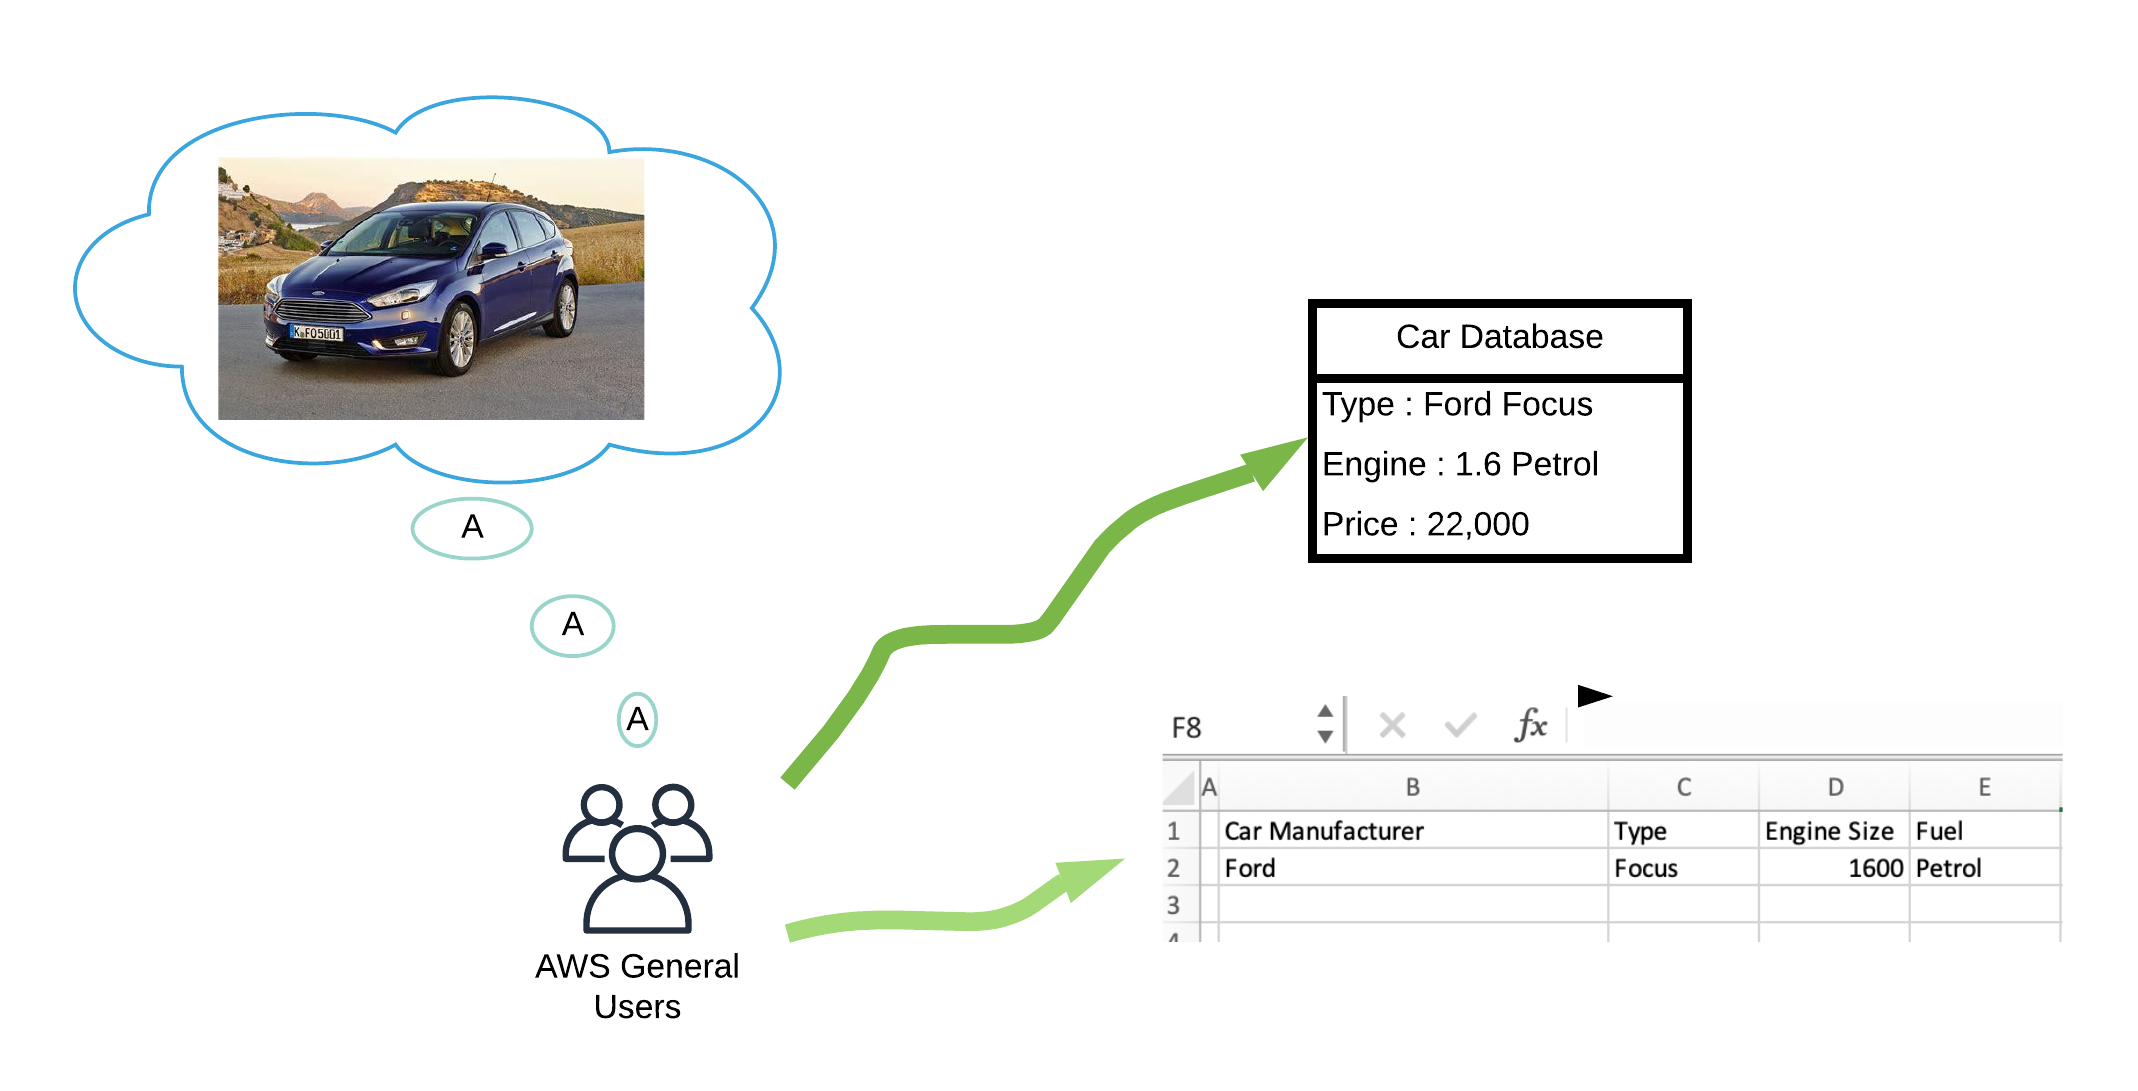
\includegraphics[scale=0.42]{Figs/datarepresentation}
%	\caption{A thing(car) in the real world represented using data}
%	\label{fig:datarep}
%\end{figure}

In practise a metadata registry is used as a means of storing this metadata.  The two core use cases that make a metadata registry essential to a data warehouse are:
\begin{enumerate}
	\item Fusing and merging datasets for analysis.
	\item Relating data elements from different sources for management.
\end{enumerate}



\subsection{Metamodel Simplification}

The purpose of an ISO11179 conformant metadata registry is to provide all the description needed to register data elements in a metadata registry. It achieves this by defining a set of artefacts around the data elements, which identify what and how the data element is used. These are terminological artefacts and they relate to the metamodel defined by the standard. The key reasons for building a metadata registry are 
\begin{itemize}
	\item to link data elements which share the same concept and thus assist with any searches for particular data elements related to a concept.
	\item to manage different versions of the same data elements 
	\item be able to identify differences between similar data elements used in different systems or programs, perhaps with similar names but different formats or data types.
	\item To manage the life cycle of data elements and sets of data elements
\end{itemize}

The current specification for ISO11179 includes a metamodel and a concept model, both of which are defined in Part 3 of the standard. The effect of applying metamodel is that models can be registered in a metadata registry, these, by definition, are models of the \emph{context} of a data element or group of data elements. This exercise looks at simplyfying the core metamodel.

The other parts of ISO11179 describe a number of different aspects of registering metadata, such as how to manage the life-cycle and versioning of metadata in a metadata registry. These aspects are not considered here, although there may be some areas which overlap.

\subsubsection{The Current ISO11179 Metamodel}

One of the key UML models in the standard shows the relationship between a data element and a data element concept, which is outlined in Part 1 of ISO11179, and the diagram on P11 - ISO/IES 11179-1:2015(E) is reproduced here in Figure~\ref{fig:dataelement}

\begin{figure}[h]
	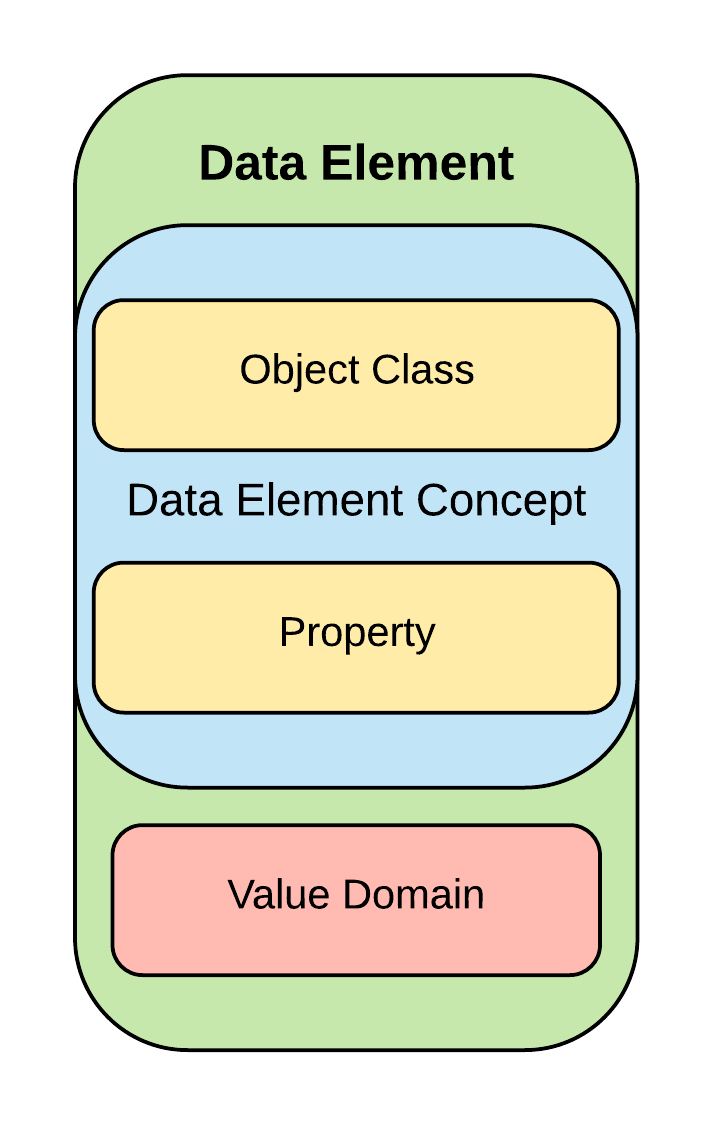
\includegraphics[scale=0.62]{Figs/DataElement1}
	\caption{Fundamental Model of Data Elements}
	\label{fig:dataelement}
\end{figure}

The idea of an object class is that it is a set of ideas which can be identied as a something about which data is collected, a grouping or classification such as vehicles, people, students, politicians, animals. It is a fairly arbitary grouping. However, the idea is that many objects in a particular class will have similar properties or characteristics, and thus a data element concept will have properties that will be shared with the data element. The Value domain becomes the part of a data element which provides representation in the real world, by assigning a value to that data element. The value may of course be textual or numerical. This set of core ideas is also expressed in Figure~\ref{fig:core}, which is derived from ISO11179-3:2013(E) Fig.11 (p93) and Fig12 (p98).

\begin{figure}[h]
	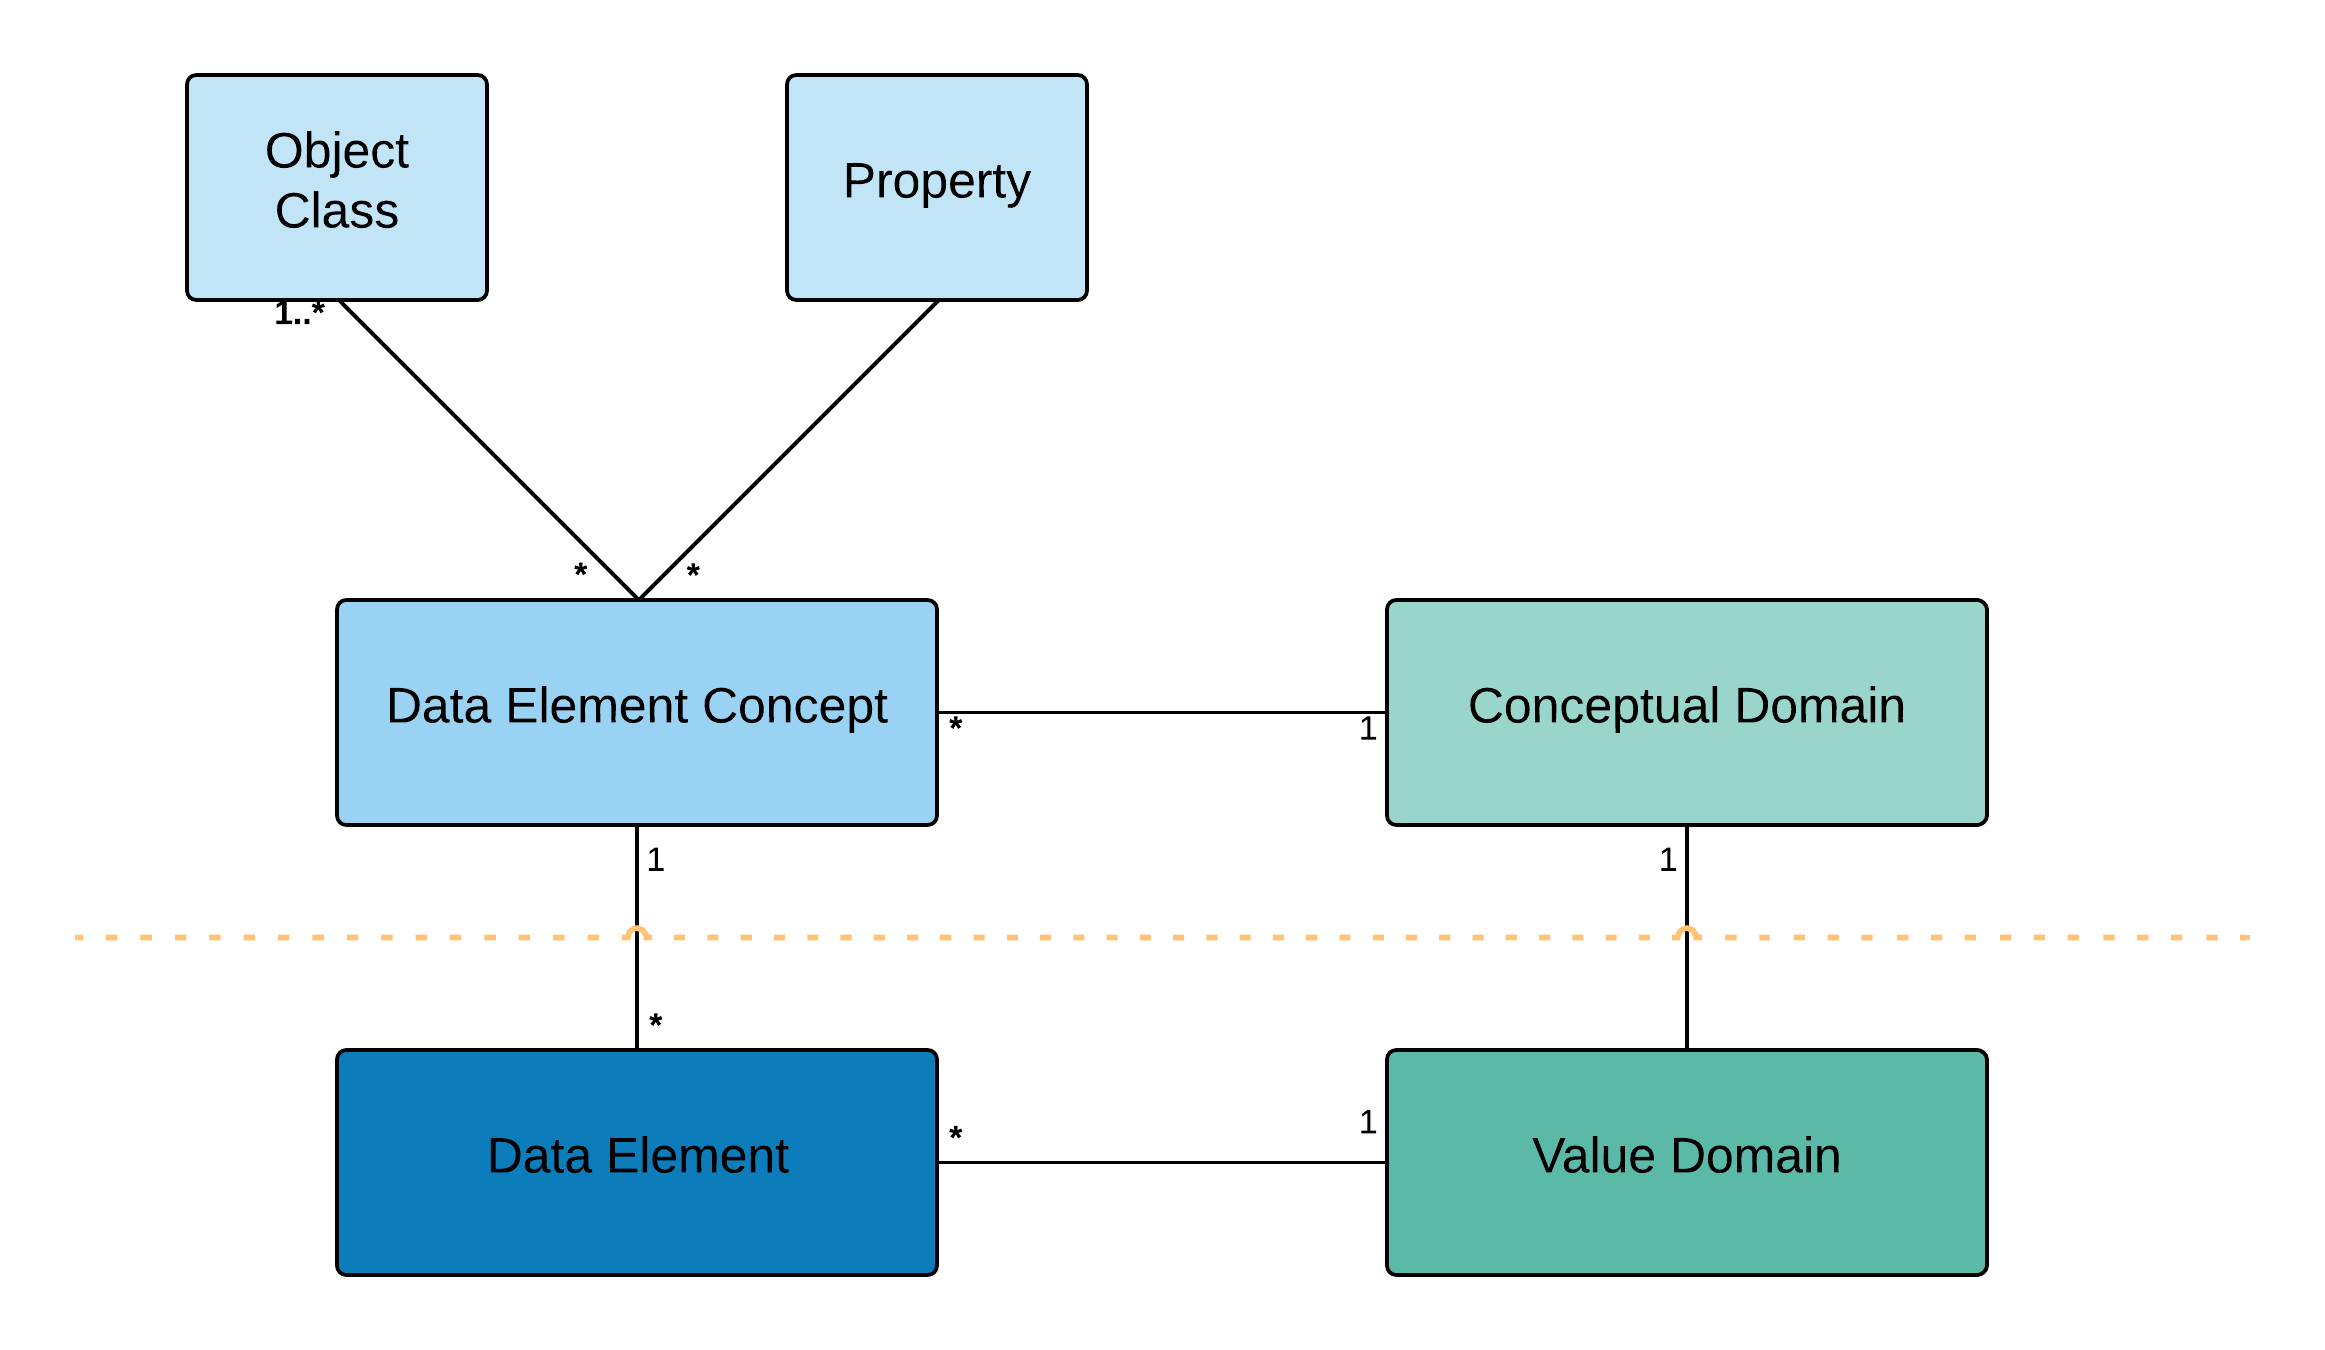
\includegraphics[scale=0.42]{Figs/ISO11179SimpleCore}
	\caption{Core Metamodel}
	\label{fig:core}
\end{figure}

The full metamodel is defined using a combination of textual description and UML diagrams. Whilst there are some examples of how to use the metamodel, or rather how to extract metadata from an example and build a conformant metamodel, there are no large-scale normative examples, tutorials or educational programs, nor is there a sample conformant registry which would be used to test different ways of building an ISO11179 conformant model. 

The metamodel is a way of describing in detail how data elements are derived from concepts and managed, however although it describes representational principles it doesn't get involved in the details. Hence the translation of the UML metamodel diagrams into a particular physical data model is left to the implementor. It is thus very much dependent on the knowledge and training of the system designer, and also on the knowledge and skill of the users who will be populating the metadata registry. 

If we look at section 9 and section 11 in terms of data modelling, section 9 could be interpreted as the Conceptual Model, and section 11 could be interpreted as the Logical Model. Using the OMG Meta object facility (MOF) section 9 could also be interpreted as a Computation Independent Model (CIM) and section 11 could be interpreted as a Platform Independent Model (PIM). In both cases the Physical Model or Platform Specific Model (PSM) is omitted. This relationship between the Physical Model and the Logical model is key, because currently there is only a one way relationship, and that is dependent on skill and interpretation.

What is needed is means of taking a Physical Model or PSM, and automatically generating the Logical Model or PIM. From there, as long as the PIM is defined in a formal manner and related to the Conceptual model in a formal manner, we can automatically build the relationships and links between data elements through the conceptual and logical models.

\subsubsection{ISO11179 Artefacts}

The standard defines a number of terms which used to build up the description of the core metamodel in Part 3, and these will be examined in the light of how one can build a model using the standard from an existing database. By taking some of the key terms, and re-defining them using a formal and a semi-formal system we can arrive at a set of definitions which can define a metamodel sufficient to capture context from any existing database or data-store.

The central artefact in the model is that of \emph{Data Element}, defined in the standard as shown in Table~\ref{tab:metamodelconstructs1}.  The definition states that it is the result of assigning a Data Element Concept to a Value Domain, and thus it is arguably a relation between a Data Element Concept and a Value Domain.


\emph{DataType} - A Datatype is designated by a data type name, and described by a datatype description. The datatype name is usually drawn from some external source, which is designated by a datatype scheme reference. Additional information may optionally be provided using the datatype annotation 

\emph{Value Domain} - An example of a Conceptual Domain and a set of Value Domains is ISO 3166, Codes for the representation of names of countries. For instance, ISO 3166 describes the set of seven Value Domains: short name in English, official name in English, short name in French, official name in French, alpha-2 code, alpha-3 code, and numeric code.

The idea of a Value Domain is not in widespread usage in data management or computer science texts, in fact it doesn't appear in a wikipedia search other than in the context of ISO11179. Thus standard representations of ISO 3166 in database tables do not include any reference to Value Domains, and it would therefore entirely feasible to represent the context in which an aspect of ISO3166 is used, say 2 character country codes, without any need to identify the Value Domain concerned. One might however wish to identify the Data Type.

Parnas~\cite{Parnas1976}  identified 5 different ways in which the word \emph{Data Type} is defined : a. Syntactic. b. Value Space. A type is defined by a set of possible values. c. Behavior. A type is defined by a value space and a set of operations on elements of that space d. Representation. A type is determined by the way that it has been represented in terms of more primitive types. 

Data Types are used in programming languages for the most part to detect errors, by having a statically and strongly typed language errors can be detected by the compiler before the program is run. Cardelli and Wegner \cite{Cardelli1985} provide the following explanation:
\begin{quotation}
A type system has as its major purpose to avoid embarrassing questions about representations, and to forbid situations where these questions might come up. In mathematics as in programming, types impose constraints which help to enforce correctness. Some untyped universes, like naive set theory, were found to be logically inconsistent, and typed versions were proposed to eliminate inconsistencies. Typed versions of set theory, just like typed programming languages, impose constraints on object interaction which prevent objects (in this case sets) from inconsistent interaction with other objects.A  type  may  be  viewed  as  a  set  of  clothes  (or  a  suit  of  armor)  that  protects  an  underlying  untyped representation from arbitrary or unintended use. It provides a protective covering that hides the underlying representation and constrains the way objects may interact with other objects. In an untyped system untyped objects are naked in that the underlying representation is exposed for all to see. Violating the type system involves removing the protective set of clothing and operating directly on the naked representation.
\end{quotation}  

Generally both programming languages and databases will have fixed datatypes, and there is a widespread degree of overlap between the many languages and databases in use, appendix 2 details the many data types in common use in C, C++, Java, Python, MySQL, SQL Server and MS Access. From this we can build up a set of artefacts which can model all these datatypes from within a metadata registry, and by defining a direct mapping we can build this part of the metadata model automatically.



\newpage 
\onecolumn	
		%\begin{table}[h]
			 \begin{table}[!htbp]
		\begin{center}
			\caption{Metamodel Domain Constructs 1}
			\label{tab:metamodelconstructs1}
			\begin{tabular}{ p{6cm} | p{8cm}  } 
				\textbf{ISO 11179 Structural Artefacts} & \textbf{Definition} \\
				\hline
				Conceptual Domain & a set of valid Value Meanings expressed as a description or via a set of enumerations   \\ 
				\hline
				Object Class &  a set of ideas, abstractions, or things in the real world that are identified with explicit boundaries and meaning and whose properties and behaviour follow the same rules     \\ 
				\hline
				Property &  a characteristic common to all members of an Object Class    \\ 
				\hline
				Data Element Concept &  A Data Element Concept is a concept that can be represented in the form of a data element, described independently of any particular representation. A Data Element Concept may have zero or one Object Class and zero or one Property. The union of a Property and an Object Class provides significance beyond either that of the Property or the Object Class. A Data Element Concept thus has a Definition independent from the Definition of the Object Class or the Property. \\
				\hline
				Data Element &   A Data Element is considered to be a basic unit of data of interest to an organization. It is a unit of data for which the definition, identification, representation, and permissible values are specified by means of a set of attributes.A Data Element is formed when a Data Element Concept is assigned a representation. One of the key components of a representation is the Value Domain, i.e., restricted valid values. \\
				\hline
				DataType & A Value Domain is associated with a Datatype — a set of distinct values, characterized by properties of those values and by operations on those values, for example the category used for the collection of letters, digits, and/or symbols to depict values of a Data Element determined by the operations that may be performed on the Data Element.
				 \\
				\hline
				Value Domain &  (3.3.140) a set of Permissible Values. One of the key components of a representation is the Value Domain. A Value Domain is associated with a Conceptual Domain. A Value Domain provides a representation for the Conceptual Domain. \\
				\hline
				Described or Non-enumerated Value Domain & A Value Domain may be expressed via a description or specification, such as a rule, a procedure, or a range (i.e., interval), rather than as an explicit set of Permissible Values. Such a Value Domain is call a Non-enumerated Value Domain. As a sub-type of Value Domain, a Non-enumerated Value Domain inherits the attributes and relationships of the former.    \\
				\hline
				Enumerated Value Domain & An Enumerated Value Domain is one where the Value Domain is expressed as an explicit set of two or more Permissible Values. As a sub-type of Value Domain, an Enumerated Value Domain inherits the attributes and relationships of the former    \\
				\hline
				Permissible Value &A Permissible Value is an expression of a Value Meaning within an Enumerated Value Domain. It is one of a set of such values that comprises an Enumerated Value Domain. Each Permissible Value is associated with a Value Meaning.   \\
				\hline
				Enumerated Conceptual Domain &  a Conceptual Domain that is specified by a list of all its Value Meanings  \\
				\hline
			\end{tabular}
		\end{center}
	\end{table}
\FloatBarrier
\begin{table*}[h]
	\begin{center}
		\caption{Metamodel Domain Constructs 2}
		\label{tab:metamodelconstructs2}
		\begin{tabular}{ p{6cm} | p{8cm}  } 
			\textbf{ISO 11179 Relational Artefacts} & \textbf{Definition} \\
			\hline
			Relation  &  A Relation is a class each instance of which models a relation (3.2.119), a sense in which concepts (3.2.18) may be connected via constituent relation roles (\\
			\hline
			Relationship & (metamodel) a connection among model elements    \\
			\hline
			Generalization & relationship (3.1.15) between a more general class (the parent) and a more specific class (the child) that is fully consistent with the general class and that adds additional information. A generalization is a type of relationship (3.1.15);
			(Adapted from ISO/IEC 19505-2:2012, 7.3.20.)\\
			\hline
			Classification & A metadata item is classified if it has one or more Classification (9.2.3.1) association classes, each with a Concept (9.1.2.1) class in a Concept System (9.1.2.2).\\
			\hline
			classification scheme &  descriptive information for an arrangement or division of objects (3.2.87) into groups based on criteria such as characteristics (3.2.14), which the objects have in common \\
			\hline
			classifiable item & metadata item (3.2.75) of a type for which classification is supported in a given metadata registry (3.2.78)\\
			\hline
			Concept System &  Concept Systems may be used as classification schemes to classify Classifiable Items within a registry, but some classification schemes will be more applicable to classifying objects in the real world than items in a registry. If the objects to be classified are not in the registry, the classification scheme may still be recorded using the Concept System structures.
			A classification scheme may be a taxonomy, a network, an ontology, or any other terminological system. The classification may also be just a list of controlled vocabulary of property words (or terms). The list might be taken from the "leaf level" of a taxonomy. Examples include SKOS, UML, OWL.   \\
			\hline
			Concept &  (3.2.18 )unit of knowledge created by a unique combination of characteristics   \\
			\hline
			Unit of measure & value domain actual units in which the associated values are measured \\
			\hline
			Dimensionality &  set of equivalent units of measure   \\
			\hline
		\end{tabular}
	\end{center}
\end{table*}
%\twocolumn
	\FloatBarrier

\newpage 
\section{Metadata Registry Federation}
		The idea behind federating metadata registries, or data catalogues is very similar to federating a database or information source, and allows users of one system to see and access all the information in the network that they have access rights to see and access.  It is not that different to having data available and accessible over the internet. 
		
		The differences arise when considering the subject matter, in this case UK tax-payer funded research datasets. Different organizations have different constraints and different ownership conditions attached to their datasets, and thus are reluctant to adopt the open linked data approach espoused by the Open Data Institute \cite[ODI]{opendata}
		
		
		Notes :  We can split the metadata defined in V2 of the HDR metadata schema into 3 main sections for the purposes of federation: summary, operational and technical.  In a linked network of metadata registries the summary metadata should be available for all registries and all users. However operational and technical metadata may have constraints placed on it, relating to the security levels of the metadata itself. For instance profiling metadata, which is part of the technical metadata, related directly to data element details, may be hidden from certain users, perhaps from other organizations, but freely available to members from the same organization.
		
		Operational: Profiling, Data Quality, Lineage(how is it captured?, processing cleaning, reference data )
		
	
		
		\subsection{Architecture}
		
		Overall the architecture is a result of what we want to achieve by the federation exercise, and also how much we can use from the pre-existing internet architectures which are already in some ways battle-hardened. One of the key issues in approaching the core architecture is the question of how we are going to move data around, how does a metadata model of dataset move from one registry instance to another? 
		
		In looking at moving metadata around there are two popular formats in use at present, JSON and XML. It may be possible to use our own metadata language for some aspects in particular the technical metadata, the problem may arise with the descriptive metadata, or more accurately the fact that it is likely to change fairly frequently.  For a fixed technical structure, based on a single metamodel, a specific \emph{domain specific language} parser, such as the MDML parser, is likely form a key element of the architecture. However with a more flexible changeable metamodel, such as this one which spans descriptive metadata, XML or JSON may be a better alternative, since this will ensure that the parser doesn't need to be rebuilt.
		
		JSON although it is in theory used more, is less verbose and has a marginally smaller footprint, is not in general any faster in terms of moving it's payload around. This appears to be due to the fact that XML has been in use longer and there are more high-performance parser in existence for XML. This is borne out by experimental measurement recording by David Lee in his paper on performance of markup languages~\cite{fatmarkup}. 
		
		XML is a languge which has been used to build up a wide range of applications over a much longer period of time than JSON, its syntax is more flexible and structured, and many of the applications and protocols which have been developed for XML can be used specifically for metadata federation. For these reasons XML is reccommended as the main language for communication and metadata transfer processes underpinning the core architecture. 
		
		
		\subsubsection{Unique Addressing}
		
		One the key issues in identifying datasets is \textbf{identification} of datasets and indeed identification of data elements themselves. As discussed in the section on \emph{Metadata Registries} data elements are at the heart of the way in which a metadata registry system works, and thus it makes sense to uniquely identify any items being registered on the federated metadata network.
		
		Standard ways of identifying data elements include using URI's, IRI's and DOI's.
		
		\paragraph{URI}
		A URI is an accronym which stands for Uniform Resource Identifier, in essence a string of characters that uniformly identifes a resource, the details of the syntax are defined in a number of internet engineeing documents and papers written by Roy Felding, Tim Berners Lee and others~\cite{uri1, uri2, uri3}. A URI is tied to a scheme, most of which use the internet domain name system as a means of ensuring uniqueness for each URI. Generally a URI is specified using 
		
		In general a URI is composed as follows:
		\begin{quote}\textbf{
				URI = scheme:[//authority]path[?query][\#fragment]
			}
		\end{quote}
		The internet standard 66 RFC3986~\cite{uri1} states:
		\begin{quote}\textbf{A Uniform Resource Identifier (URI) is a compact sequence of characters that identifies an abstract or physical resource. This specification defines the generic URI syntax and a process for resolving URI references that might be in relative form, along with guidelines and security considerations for the use of URIs on the Internet. The URI syntax defines a grammar that is a superset of all valid URIs, allowing an implementation to parse the common components of a URI reference without knowing the scheme-specific requirements of every possible identifier. This specification does not define a generative grammar for URIs; that task is performed by the individual specifications of each URI scheme..}
		\end{quote}
	
	    The URI scheme is used in semantic web technologies to identify both concepts and documents, and is used by XML to define namespaces.XML 1.1 has replaces UIR's with IRI's.
	    
	    \paragraph{IRI}
	    Internationalized Resource Identifier''s (IRI) are effectively URI's, except that they are using the Universal Character set (e.g. UTF-8), as opposed to ASCII, which is specified for URI's. They were introduced to allow international users to access internet resources using a variety of character sets. The intention is that over time IRI's will replace URI's as the main system for recourse identification.  The IRI was specified by the internet standard RFC3987~\cite{iri1}.
	    
	    \paragraph{URN}
	    A Uniform Resource Name (URN) is a URI that identifies a resource by name in a particular namespace, it differs from a URL in that it doesn't have information about it's location or how to access it. To quote from~\cite{urn1}:
	    
	    \begin{quote}\textbf{URL is a useful but informal concept: a URL is a type of URI that identifies a resource via a representation of its primary access mechanism (e.g., its network "location"), rather than by some other attributes it may have.}
	    \end{quote}
	    
	    \paragraph{URL}
		Tim Berners-Lee proposed Unified Resource Locators in a paper published in 1994~\cite{url1} and published by the World Wide Web Consortium, as a means of identifying web resources, and by using the domain name service, using the unique name as a means of de-referencing them. They are used throughout the internet, and are very much written into the way the world wide web works. They follow the syntax specified by the URI specification, and can be thought of as a specialised form of URI.
		
			
		\paragraph{DOI}

		A digital object identifier is an identifier for any kind of digital object as specified by the Digital Organisation Foundation(DOF), an organisation set up to promote DOI's. ISO published a standard around DOI's, ISO 26324 ~\cite{doi1} DOI's are registered by organisations that maintain registries on behalf of DOF, some of these are government and some like \emph{DataCite} are specialised around specific user communities. The registries enable users to see what documents, or datasets are available from other users, by storing metadata about the digital object. 
		
		The ISO DOI scheme which is managed by the Digital Organisation Foundation is based on the Handle system pioneered by Corporation for National Research Initiatives (CNRI) who run the Handle.Net Registry (HNR).
		
		
		\subsubsection{Presence}
		A federated system will need a mechanism for each registry to announce its presence on the network.
		
		\subsubsection{Structured Data}
		A federated system needs the ability to exchange structured data, and to validate that data when it is received. A schema or meta-model, as specified in the descriptive metadata section, will be needed to specifiy this data.
		
		
		\subsubsection{Federated Client/Server}
		Each registry is in essence a server, it will announce it's presence, and respond to requests from other servers as appropriate. Clients, such as web browsers, will be able to connect directly to different servers according to a configuration setup.
		
		
		\subsection{Network Binding}
		Federation in the context of healthcare datasets implies that any protocol needs to be bound to the internet, either by binding directly to TCP or by using HTTPS/TLS as the main mechanism for metadata interoperability.
		
		\subsubsection{Fully Qualified Domain name resolution}
		One of the core mechanism's for moving data around the internet is the domain name resolution service, which enables URL's to map to IP address's, using both IP4 and IP6. 
		
		The fully qualified domain name service (FQDN) works to resolve from a URL a service which is available on a particular port and ip address, in essence the following process is followed in order to open a connection between a server and a client over TCP (or another protocol).
		\begin{enumerate}
			\item An entity build up a DNS SRV query, consisting of service requirement, the transport protocol (e.g. TCP), and the target.
			\item A response is received ideally containing one or more details of services running, which will either cause the initator to continue or abort
			\item The initiator chooses one of the services, and then resolves the URL, receiving back an ip address.
			\item The initiator either opens a connection to the service on that ip address, or aborts.
		\end{enumerate}
		
		\subsubsection{Reliability}
		Sending large payloads over TCP connections is inherently unreliable, thus many services seek to enhance the core capability with various checks on transmission and reception so that large payloads, such as XML or XSD files		
		
		\subsection{XML and XMPP Transport}
		XMPP is the Extensible Messaging and Presence Protocol, and fullfills all the main requirements for building a federated registry system for metadata. The basic mechanisms for moving XML messages around the internet are well established, and form the basis for services such Google's hangouts and other messaging services. It has the capability to work on the existing domain name system, 
		\subsection{Security}
		\subsubsection{Consent}
		
		\section{Appendix A}
		\subsection{MDML}
		This subsection defines the MetaData Modelling Language (MDML). The work has been informed by work carried out with Genomics England in standardising dataset for use in research in conjunction with patients genetic profiles. During these studies it was observed that despite the existance of many separate standards, there are still huge barriers to interoperability within the UK NHS. As a result work was undertaken to address the following specific issues:
		\begin{itemize}
			\item  Standard description of data, and how to manage and maintain data standards.
			\item Common understanding of data across organizational elements and between organizations
			\item Re-use and standardization of data over time, space, and applications
			\item Harmonization and standardization of data within an organization and across organizations
			\item Management of the components of data
			\item Re-use of the components of data
		\end{itemize}
		
		The need to capture data structures, relationships, and rules suggests that our language should have the core features of an entity-relationship or object modelling notation, and the ability to express logical constraints on values and value sets.  The Unified Modeling Language (UML) is a widely-used notation which meets this basic requirement, and could be an ideal starting point for our language definition. 
		
		UML has a stereotype mechanism built in for the definition of languages and profiles, however, as is pointed out in~\cite{stereouse} the UML Stereotype mechanism is difficult to use effectively and open to mis-interpretation. Furthermore, Briand and Williams in Model Driven Engineering Languages and Systems~\cite{modtools} argue convincingly that the stereotype mechanism in UML 2.0 is lacking in expression and is not as powerful as having another meta-layer in the modelling toolkit.  Nierstrasz, Whittle, Harel and Reggio~\cite{ustereo} demonstrate in \emph{"Uses and Abuses of the Stereotype Mechanism in UML 1.x and 2.0"} that the stereotype mechanism introduced in UML 2.0 is incompatible with set theory, and does not allow a useful semantic interpretation in terms of constraints.
		
		For these reasons, a different approach to the definition of the language is taken. The abstract language syntax and constraint semantics are specified using the Z notation, following which a concrete implementation of the language using the XText~\cite{XText} toolkit of the ECore/EMF modelling framework~\cite{ECORE}.  ECore may be seen as a widely-used implementation of the UML MOF standard---for the purposes of data language definition, there are no significant differences between the two---and comes with a range of widely-used visualisation,programming and modelling tools. Why not use Ecore without defining a separate language? Initially, this work evolved from research into the ISO standard for metadata registries: ISO11179, and in particular the metamodel described in part 3 of this standard. This specifies a metamodel and a model for a metadata registry, however it is a very complicated definition. This work is an attempt to take the essentials, simplify them and make the standard one which can be applied by machines and humans alike.
		
		
		\section{MDML - Abstract Specification.}
		
		This needs work on the requirements from the Data Type Registry work.....
		
		The language needs to define data elements, ways to group data elements, and ways to handle relationships between different elements, within the same domain or collection, and with data elements in other collections. It also needs to be able to define rules, for typing and thus verifying data items, and also to define rules or constraints, which in turn operate on groups of data elements. By defining constraint information within one group, that information then has the possibility to be transferred with the data during data transfer operations, or due to the reference mechanisms in place to be referred to at a later point in time.
		
		By considering atomic data-items as data elements, and by considering groups of data elements as data classes, a basic data structure, corresponding to the structure used in almost all object oriented computer languages can be built up. Groups of classes are termed models, a model corresponding to a dataset, or as in the case of health informatics a data standard such as FHIR~\cite{FHIR}
		
		Two basic types allow the representation of textual information and numeric data values:
		\begin{zed}
			[Text, Value]
		\end{zed}
		In this initial version of the language no attempt is made at defining constraint information in the language, it is sufficient to capture it in a textual form.
		
		Some values, subject to a constrained syntax, can be used as names for dataitems.  A particular set of values will be used as identifiers, including implicit identifiers within models. While developing a model it's composition and structure are going to be \emph{mutable}, however once a model is agreed, it needs to become \emph{immutable} or \emph{finalised}.  A finalised model will have a fixed, externally-valid name: a globally-unique identifier, this will enable any references to be used in automatic processes in a reliable and robust fashion. 
		
		Currently most published data standards do not have any globally-unique identifier which can be used by heterogeneous systems in different locations to refer to during any shared operation or communication. This requirement, for a common point of reference for different systems, indicates that the language will become a key part of a defining a metadata registry, a registry to contain data definitions for many differing datasets or models, unlike a data dictionary, which simply defines the datasets being used within a specific relational database.
		
		\begin{axdef}
			Name, Id, GUID : \power Value 
		\end{axdef}
		An implicit reference to another item within the same model is achieved using a single identifier.  Explicit references beyond a model will require instead the resolution of a path: a sequence of names of models, classes, and other components:
		\begin{syntax}
			Path == \seq Name 
		\end{syntax}
		A finalised item in a registry or catalogue can be accessed using a published path.  Such a path will begin with the name of a finalised data model (see below); this will be followed by a sequence of names identifying an item declared within that model or, if the sequence is empty, the model itself. 
		
		%		Every item declared within a model, and the model itself, will have a name, a textual description, and two possibly-empty sets of paths: sequences of names that uniquely identify items in this or other models.  The first of these sets, $refines$, is used to record assertions of semantic refinement:  assertions that every instance of this item will satisfy every property mentioned in the declarations of the others.
		%		
		%		The second set, $doesNotRefine$, is used to record assertions of non-refinement. The same path $p$ will not appear in both $refines$ and $doesNotRefine$ for the same item, furthermore the absence of $p$ from one of these attributes does not imply its presence in the other.  This can be considered to be an `open world' property. 
		
		Each item in a model will be represented by an instance of a schema extending the following declaration:
		\begin{schema}{DataItem}
			name : Name \\
			text : Text \\
			id : Id \\
			refines, doesNotRefine : \power Path
		\end{schema}
		Thus every item has a unique identifier.
		
		The type of data item may be a basic primitive type, enumeration, or a reference to an instance of a class: the latter gives a mechanism for describing relationships between entities modelled as classes.
		
		A primitive type has as a set of values, and is represented as an instance of the following schema:
		\begin{schema}{Primitive}
			DataItem \\
			values : \power Value 
		\end{schema}
		An enumeration has a set of names or terms, each of which may be associated with a textual explanation.
		
		A key consideration in the language design is that it should be possible to express intended semantic relationships without the need for a separate, external ontology. In effect, the model can be considered as an ontology, since each data item is represents a concept which is related to other concepts.  
		
		%		For this reason, any component of a data model that has a textual explanation, or natural language definition, should have a $refines$ attribute, allowing it to draw some or all of this explanation from an existing component, and providing a basis for automatic determination of semantic interoperability. The $refines$ attribute could be informally equated with the terms \emph{based on} or \emph{derived}, which are terms that crop up currently in healthcare related data standards.
		
		Accordingly, the individual terms of an enumeration are managed items in their own right.
		\begin{schema}{Enum}
			DataItem 
		\end{schema}
		They have no additional properties or context: they are simply terms appearing in an enumeration.   An enumeration is itself a definable (and hence refine-able) item. 
		\begin{schema}{Enumeration}
			DataItem \\
			enum : Name \pfun Enum
			\where
			\forall n : \dom enum \spot (enum~n).name = n 
		\end{schema}
		The representation of the set of $Enum$ items as a function on names is partly a matter of notational convenience: the constraint insists that the naming is consistent with the $name$ property of each member. It also expresses the property that each name is unique: the relationship between names and enumerations is functional. 
		
		In addition to a type, a data item has a name, a textual definition, a multiplicity, and an ordering.  A multiplicity is either optional, mandatory, or many-valued:
		\begin{syntax}
			Multiplicity & ::= & \optional \mid \mandatory \mid \many 
		\end{syntax}
		and a many-valued item can be either ordered or unordered:
		\begin{syntax}
			Ordering & ::= & ordered \mid notOrdered 
		\end{syntax}
		The type itself is represented as a reference, as an identifier, as many data items may share the same type. 
		
		A data item is then represented as an instance of the following schema: 
		\begin{schema}{DataItem}
			DataItem \\
			multiplicity : Multiplicity \\
			ordering : Ordering \\
			type : Name
		\end{schema}
		The type of a data item must be declared within the current data model, or within one of the models that it imports: see below. 
		
		A class has a set of members, each a named data item.  It has also a name, a textual definition, and a constraint.  There are two notions of factorisation in class declarations, both of which should be familiar from object modelling: a class may `contain' other classes, corresponding to an extension of scope or control in implementation; a class may also `extend' other classes, in the sense of extending or re-using an existing class declaration.  These other classes are declared at the same level, and thus the connections to them are represented using identifiers.
		
		A data class is represented by the following schema:
		\begin{schema}{DataClass}
			DataItem \\
			contains, extends : \power Path \\
			members : Name \pfun DataItem
			\where
			\forall n : \dom members \spot (members~n).name = n 
		\end{schema}
		Names are unique within a model. A model has a name, a textual definition, and an identifier.  It may import the contents of other models.  It contains a set of classes, enumerations, and primitive types: every class, enumeration, or primitive that we will consider is declared in exactly one model.  It has a status, indicating whether or not it has been finalised: this is a key distinction, as only finalised or immutable models may be used as a basis for determining interoperability.  As mentioned before, finalised models will be allocated a globally-unique identifier.
		\begin{syntax}
			Status & ::= & draft \mid final 
		\end{syntax}
		It has also a constraint (which may be empty, or $true$). 
		
		A data model is represented by the following schema:
		\begin{schema}{Model}
			DataItem \\
			imports : \power Name \\
			classes : Name \pfun DataClass \\
			enumerations : Name \pfun Enumeration \\
			primitives : Name \pfun Primitive \\
			status : Status
			\where
			\forall n : \dom classes \spot (classes~n).name = n \\
			\forall n : \dom enumerations \spot (enumerations~n).name = n \\
			\forall n : \dom primitives \spot (primitives~n).name = n 
		\end{schema}
		Names of classes, enumerations, and primitives must be unique within a model.
		
		The end goal is to simplify interoperability by using linked collections of data models, maintained in a (possibly-distributed) metadata registry or catalogue.  The language can be extended to include the description of a registry,which can then capture the constraint information that exists across models: the uniqueness of the identifiers, the integrity of implicit referencing, and the fundamental impact of versioning upon data model development and re-use.
		
		A metadata registry is an administered collection of data models, subject to specific constraints upon the way in which models are created, edited, and published.  For the purposes of this chapter, a registry or catalogue may be represented as an instance of (a subtype of) the following schema:
		\begin{schema}{Collection}
			models : Name \pfun Model
		\end{schema}
		Model names are unique within a collection. 
		%\bibliographystyle{ieeetran}apalike
	\bibliographystyle{ieeetran}
{\small
	\bibliography{datatype}}


\end{document}

